%\documentclass[10pt]{beamer}  % pour la présentation
\documentclass[10pt,handout]{beamer}  % pour les notes de cours


\usetheme{Antibes}
\usecolortheme{whale}
\setbeamertemplate{navigation symbols}{}
\setbeamertemplate{mini frames}{} % Supprime les petits cercles dans le header
\setbeamertemplate{items}[triangle]
\setbeamercolor{itemize item}{fg=black}
\setbeamercolor{itemize subitem}{fg=gray}


\usepackage[utf8]{inputenc}
\usepackage[T1]{fontenc}
\usepackage[english]{babel}
\usepackage{amsmath, amssymb}
\usepackage{hyperref}
\usepackage{graphicx}
\usepackage{caption}
\usepackage{tikz}
\usetikzlibrary{shapes.geometric, positioning}
\usepackage{nicematrix}


\title{Machine Learning - L3 - KMAXPP05}
\subtitle{Chapter 1 : Foundations of Machine Learning}
\author{Cédric Campguilhem}
\institute[]{
	Airbus Operations \\
	\href{mailto:cedric.campguilhem@airbus.com}{\texttt{cedric.campguilhem@airbus.com}}
}
\date{2025-2026}

\begin{document}

\begin{frame}
  \titlepage
\end{frame}

\section[Introduction]{Introduction}

\subsection[Course Organization]{Course Organization}

\begin{frame}{Course Organization}
	The course is organized around:
	\begin{itemize}
		\item Lectures: 20 hours (2h x 10 sessions)
		\item Tutorials: 16 hours (2h x 8 sessions)
		\item Practical sessions: 20 hours (2h x 10 sessions)
	\end{itemize}
	\vspace{0.5cm}
	The following time slots will be used:
	\begin{itemize}
		\item Tuesday 15:45 - 17:45: Tutorials / Practical sessions
		\item Tuesday 18:00 - 20:00: Exams
		\item Thursday 13:30 - 15:30: Lectures / Practical sessions
	\end{itemize}
\end{frame}

\begin{frame}{Assessments}
	\begin{tabular}{|l|l|l|l|l|}
		\hline
		\textbf{Item} & \textbf{\%} & \textbf{Duration} & \textbf{Format} & \textbf{Date} \\
		\hline
		CC1 & 33\% & 20 min & In-class, MCQ & 19/03 \\
		\hline
		TD \& TP & 33\% & - & Attendance, lab completion, project & - \\
		\hline
		CC3 & 34\% & 1h30 & Exam conditions & 19/05 \\
		\hline
		CC4 & - & 1h30 & Exam conditions & 11/06 \\
		\hline
	\end{tabular} \\
	\vspace{0.5cm}
	Note: The CC3 exam will take place during the Tuesday 18:00 - 20:00 slot.
\end{frame}

\begin{frame}{Course Outline}
	\begin{itemize}
		\item Foundations of Machine Learning [6h]
		\begin{itemize}
			\item Introduction
			\item Typology of Machine Learning Problems
			\item Core Issues in Artificial Learning
			\item Linear Models
			\item Validation of Machine Learning Algorithms
		\end{itemize}
		\item Machine Learning Algorithms [13h30]
		\begin{itemize}
			\item Naïve Bayes Algorithm [1h30]
			\item Principal Component Analysis [2h]
			\item Decision Trees [2h]
			\item Perceptrons and Multilayer Perceptrons [4h]
			\item K-Means [2h]
			\item K-Nearest Neighbors [2h]
			%\item Support Vector Machines [4h]%
		\end{itemize}
	\end{itemize}
\end{frame}

\subsection[Paradigms]{Paradigms}

\begin{frame}{Paradigms and Systems of Thought}
	Daniel Kahneman (2002 Nobel Prize in Economics) theorized 2 modes of functioning of the human brain:
	\begin{itemize}
		\item \textbf{Slow thinking}: conscious, logical, effortful
		\item \textbf{Fast thinking}: unconscious, intuitive, effortless
	\end{itemize}
	\vspace{0.5cm}
	\begin{columns}
		\begin{column}{0.5\textwidth}
			\begin{figure}
				\centering
				\includegraphics[height=0.5\linewidth]{Images/velo_centrifuge}
				\label{fig:velo-centrifuge}
			\end{figure}
			%\vspace{-0.5cm}
			\centering
			\small Logical approach
		\end{column}
		\begin{column}{0.5\textwidth}
			\begin{figure}
				\centering
				\includegraphics[height=0.5\linewidth]{Images/velo-t-es-capable}
				%\caption{approche intuitive}
				\label{fig:velo-t-es-capable}
			\end{figure}
			%\vspace{-0.5cm}
			\centering
			\small Intuitive approach
		\end{column}
	\end{columns}
	\vfill 
	\tiny \textcolor{gray}{Source: Thinking, fast and slow - D. Kahneman - 2012 - Penguin}
\end{frame}

\begin{frame}{Paradigms and Systems of Thought}
	A link can be established with programming paradigms:
	\begin{itemize}
		\item Slow thinking $\rightarrow$ \textbf{Deductive} programming: based on logical and explicit rules, derived from human knowledge. The program applies the rules to the provided data.
		\item Fast thinking $\rightarrow$ \textbf{Inductive} programming: based on data and experience; the rules are implicit and discovered by the algorithm. The program applies the rules it has discovered to new data; it generalizes.
	\end{itemize}
\end{frame}

%\begin{frame}{Paradigms and Systems of Thought}
%	Nevertheless, another paradigm exists:
%	\begin{itemize}
	%		\item Mimicry $\rightarrow$ \textbf{Transductive} programming: there are no rules, implicit or explicit, independent of the training data. The algorithm does not generalize, it copies.
	%	\end{itemize}
%	\begin{figure}
	%		\centering
	%		\includegraphics[height=0.3\linewidth]{Images/mimétisme}
	%		\label{fig:mimétisme}
	%	\end{figure}
%	%\vspace{-0.5cm}
%	\centering
%	\small Mimetic approach
%\end{frame}

\subsection[Definitions]{Definitions}

\begin{frame}{Definitions of Machine Learning}
	\begin{block}{Definition 1}
		Field of study that gives computers the ability to learn without being explicitly programmed. \\
		\hfill
		\textit{--- Arthur Samuel (1959)}
	\end{block}
	\vfill
	\tiny \textcolor{gray}{Source: Some Studies in Machine Learning Using the Game of Checkers - A.L. Samuel - 1959 - IBM Journal}
\end{frame}

\begin{frame}{Definitions of Machine Learning}
	\begin{block}{Definition 2}
		A program learns from \textbf{experience $E$} for a \textbf{task $T$} with a \textbf{performance $P$}, if $P$ improves with $E$. \\
		\hfill 
		\textit{--- Tom Mitchell (1997)}
	\end{block}
	%\pause
	\begin{itemize}
		\item \textbf{Experience ($E$)} = Data.
		\item \textbf{Task ($T$)} = Predict, classify, cluster, act, generate.
		\item \textbf{Performance ($P$)} = The mathematical loss function.
	\end{itemize}
	\vfill 
	\tiny \textcolor{gray}{Source: Machine Learning - T.M. Mitchell - 1997 - McGraw-Hill}
\end{frame}

\begin{frame}{Everything is a number!}
	\begin{figure}
		\centering
		\includegraphics[width=1.0\linewidth]{Images/tout_est_nombre}
		\label{fig:tout-est-nombre}
	\end{figure}
\end{frame}
\section[Typology]{Typology of Machine Learning Problems}

\begin{frame}{Machine Learning}
	We can distinguish 3 major families of machine learning algorithms:
	\begin{itemize}
		\item \textbf{Unsupervised} learning
		\item \textbf{Supervised} learning
		\item \textbf{Reinforcement} learning
	\end{itemize}
\end{frame}

\subsection[Unsupervised Learning]{Unsupervised Learning}

\begin{frame}{Unsupervised Learning}
	From a sample of observations $\mathcal{D} = \begin{Bmatrix}x^{(1)}, x^{(2)}, \cdots, x^{(n)}\end{Bmatrix}$, the goal of an unsupervised learning algorithm is to discover the \textbf{internal structure} of the data. This can be achieved by:
	
	\begin{itemize}
		\item Grouping together observations that share similar characteristics: \textbf{clustering}
		\item Finding a simplified representation of the observations with a reduced number of features: \textbf{dimensionality reduction}
	\end{itemize}
	\vspace{0.5cm}
	There is, a priori, no specific expected response from the algorithm.
	
\end{frame}

\begin{frame}{Unsupervised Learning}
	Here are a few examples of algorithms:
	
	\begin{itemize}
		\item Clustering:
		\begin{itemize}
			\item K-Means algorithm: \href{https://scikit-learn.org/stable/modules/generated/sklearn.cluster.KMeans.html}{\texttt{sklearn.cluster.KMeans}}
			\item DBSCAN (Density-Based Spatial Clustering of Applications with Noise): \href{https://scikit-learn.org/stable/modules/generated/sklearn.cluster.DBSCAN.html}{\texttt{sklearn.cluster.DBSCAN}}
		\end{itemize}
		\item Dimensionality reduction:
		\begin{itemize}
			\item Principal Component Analysis (PCA): \href{https://scikit-learn.org/stable/modules/generated/sklearn.decomposition.PCA.html}{\texttt{sklearn.decomposition.PCA}}
			\item t-SNE (t-Distributed Stochastic Neighbor Embedding): \href{https://scikit-learn.org/stable/modules/generated/sklearn.manifold.TSNE.html}{\texttt{sklearn.manifold.TSNE}}
		\end{itemize}
	\end{itemize}
\end{frame}

\begin{frame}{Example of Unsupervised Learning}
	Consider the following data for rugby players:
	\begin{table}
		\centering
		\begin{tabular}{|c|c|c|c|}
			\hline
			\textbf{Height} (cm) & \textbf{Weight} (kg) & \textbf{Age} & \textbf{Number of caps} \\ \hline
			190              & 112            & 29           & 47 \\
			172              & 85             & 22           & 5  \\
			186              & 135            & 37           & 0  \\
			180              & 92             & 30           & 70 \\
			\hline
		\end{tabular}
	\end{table}
	\begin{itemize}
		\item A clustering algorithm could, for example, group the tallest and heaviest players together, or those with the highest number of caps.
		\item A dimensionality reduction algorithm could, for example, take advantage of the correlation between height and weight on one hand, and age and number of caps on the other, to propose a simplified representation based on only 2 features, respectively: build and experience.
	\end{itemize}
\end{frame}

\subsection[Supervised Learning]{Supervised Learning}

\begin{frame}{Supervised Learning}
	From a sample of observations $\mathcal{D} = \begin{Bmatrix}(x^{(1)}, y^{(1)}), (x^{(2)}, y^{(2)}), \cdots, (x^{(n)}, y^{(n)})\end{Bmatrix}$, the goal of a supervised learning algorithm is to discover the \textbf{relationship} linking the input features ($x$) to the output features ($y$). \\
	\vspace{0.5cm}
	Two families stand out based on the continuous or discrete nature of the output features:
	\begin{itemize}
		\item \textbf{Regression} algorithms: when the output features represent a continuous value
		\item \textbf{Classification} algorithms: when the output features represent a discrete value
	\end{itemize}
	\vspace{0.5cm}
	There is, a priori, a precise expected response from the algorithm.
\end{frame}

\begin{frame}{Example of a Regression Problem}
	Staying with our rugby players example:
	\begin{table}
		\centering
		\begin{tabular}{|c|c|c|c|}
			\hline
			\textbf{Height} (cm) & \textbf{Weight} (kg) \\ \hline
			190              & 112 \\
			172              & 85  \\
			186              & 135 \\
			180              & 92  \\
			\hline
		\end{tabular}
	\end{table}
	A supervised learning algorithm could, for example, find a relationship between a player's height and weight. This would allow us to \textbf{predict} the weight of a rugby player not listed in this experiment, based purely on their height.
\end{frame}

\begin{frame}{Example of a Classification Problem}
	Never change a winning team:
	\begin{table}
		\centering
		\begin{tabular}{|c|c|c|c|}
			\hline
			\textbf{Height} (cm) & \textbf{Weight} (kg) & \textbf{Position} \\ \hline
			190              & 112 &  Back row       \\
			172              & 85  &  Fly-half \\
			186              & 135 &  Prop           \\
			180              & 92  &  Centre           \\
			\hline
		\end{tabular}
	\end{table}
	A supervised learning algorithm could, for example, find a relationship between a player's height and weight on one hand, and their position on the other. This would allow us to \textbf{predict} the position of a rugby player not listed in this experiment, based on their height and weight.
\end{frame}

\subsection[Reinforcement Learning]{Reinforcement Learning}

\begin{frame}{Reinforcement Learning}
	Unlike the previous modes, reinforcement learning does not rely on a fixed data sample but on dynamic \textbf{interactions}. \\
	\vspace{0.5cm}
	An \textbf{agent} operates within an \textbf{environnement} and must learn to make \textbf{sequential} decisions:
	\begin{itemize}
		\item The agent observes a \textbf{state} (the current context)
		\item It chooses an \textbf{action} to execute
		\item It receives a \textbf{reward} (positive or negative, immediate or deferred) in return
	\end{itemize}
	\vspace{0.5cm}
	The goal of the algorithm is to discover the \textbf{optimal strategy} to maximize the total long-term reward. \\
	\vspace{0.5cm}
	There is, a priori, no specific expected response from the algorithm. However, it is possible to precisely evaluate the quality of its answer.
\end{frame}

\begin{frame}{Example of Reinforcement Learning}
	In the example below, we can see how an agent interacts with its environment (the car and the track) through its sensors and actions performed on the vehicle's steering and speed. The objective is to find an optimal trajectory (position and speed) to minimize lap time without leaving the track (penalty):
	\begin{columns}
		\begin{column}{0.5\textwidth}
			\begin{figure}
				\centering
				\includegraphics[height=0.6\linewidth]{Images/autonomous_car1}
				\label{fig:autonomous-car-1}
			\end{figure}
			\vspace{-0.3cm}
			\centering
			\small The agent's interactions
		\end{column}
		\begin{column}{0.5\textwidth}
			\begin{figure}
				\centering
				\includegraphics[height=0.6\linewidth]{Images/autonomous_car2}
				\label{fig:autonomous-car-2}
			\end{figure}
			\vspace{-0.3cm}
			\centering
			\small Optimal strategies
		\end{column}		
	\end{columns}
	\vfill 
	\tiny \textcolor{gray}{Source: Comparing deep reinforcement learning architectures for autonomous racing - B.D Evans, H.W. Jordaan, H.A Engelbrecht - Elsevier 2023}
\end{frame}

%\subsection[Methods]{Methods}
%
%\begin{frame}<0>{Parametric and Non-Parametric Methods}
%	There is another way to categorize machine learning algorithms:
%	\begin{itemize}
	%		\item \textbf{Parametric} methods: The algorithm has a \textbf{fixed} number of parameters, independent of the size of the training sample. The algorithm \textbf{summarizes} the training data.		
	%		\item \textbf{Non-parametric} methods: The algorithm has a \textbf{variable} number of parameters, depending on the sample size. The algorithm \textbf{adapts} its structure to the training data.
	%	\end{itemize}
%\end{frame}
%
%\begin{frame}<0>{Example of Parametric and Non-Parametric Methods}
%	Using the same data as before:
%	\begin{table}
	%		\centering
	%		\begin{tabular}{|c|c|c|c|}
		%			\hline
		%			\textbf{Height} (cm) & \textbf{Weight} (kg) & \textbf{Position} \\ \hline
		%			190              & 112 &  Back row       \\
		%			172              & 85  &  Fly-half \\
		%           186              & 135 &  Prop           \\
		%			180              & 92  &  Centre           \\
		%			\hline
		%		\end{tabular}
	%	\end{table}
%	We could imagine an algorithm that predicts the position of a player of a given height and weight (for example, 185 cm and 95 kg) based on the observation in the training data that is closest to this player's characteristics. Proximity can be evaluated using a Euclidean norm.
%\end{frame}
%
%\begin{frame}<0>{Example of Parametric and Non-Parametric Methods}
%	Here, the algorithm would predict the position as "centre". To support its prediction, the algorithm relies directly on the training data without resorting to the generalization of a rule. The internal structure of the algorithm is directly the training data itself, and it becomes more complex as the number of observations grows. This algorithm is both \textbf{transductive} (there is no explicit prediction function independent of the data) and \textbf{non-parametric}. \\
%	\vspace{0.5cm}
%	An extremely similar algorithm will be studied in this course: the K-Nearest Neighbors algorithm.
%\end{frame}
%
%\begin{frame}<0>{Example of Parametric and Non-Parametric Methods}
%	Focusing now solely on height and weight:
%	\begin{table}
	%		\centering
	%		\begin{tabular}{|c|c|c|c|}
		%			\hline
		%			\textbf{Height} (cm) & \textbf{Weight} (kg) \\ \hline
		%			190              & 112 \\
		%			172              & 85  \\
		%			186              & 135 \\
		%			180              & 92  \\
		%			\hline
		%		\end{tabular}
	%	\end{table}
%	An algorithm could predict a player's weight knowing their height. This is typically what a linear regression can achieve:
%
%	\begin{equation}
	%		\text{weight} = \beta_0 + \beta_1 \times \text{height}
	%		\nonumber
	%	\end{equation}
%	
%	Here, the algorithm only has two parameters, $\beta_0$ and $\beta_1$, regardless of the number of observations. It is both \textbf{inductive} and \textbf{parametric}.
%	
%\end{frame}
%
%\begin{frame}<0>{Example of Parametric and Non-Parametric Methods}
%	\begin{itemize}
	%	\item A learning algorithm can be both \textbf{inductive} and \textbf{non-parametric}. Gaussian Processes are an example of an algorithm that meets both criteria. A Gaussian Process builds a covariance matrix from the observed data. The Gaussian Process summarizes the interdependencies of the training data within this covariance matrix (inductive nature). However, the rank of the covariance matrix grows with the number of observations, and the output features of the training data remain required for prediction (non-parametric nature).
	%	\item There are algorithms that are both \textbf{transductive} and \textbf{parametric}, such as transductive support vector machines. However, these algorithms remain quite rare.
	%	\end{itemize}
%\end{frame}
\section[Problem Statement]{Problem Statement}
\begin{frame}{Problem Statement}
	In this section, we will introduce fundamental concepts of supervised learning:
	\begin{itemize}
		\item The hypothesis space
		\item The hierarchy of learning spaces
		\item The formulation of regression and classification problems
	\end{itemize}
\end{frame}

\subsection[Spaces]{Hypothesis and Learning Spaces}

\begin{frame}{Hypothesis Space}
	Let $\mathcal{X}$ and $\mathcal{Y}$ be, respectively, the input space and the output space available for our supervised learning problem.
	\begin{block}{Hypothesis: True Function $f$}
		We assume there exists a \textbf{true} but unknown function $f: \mathcal{X} \rightarrow \mathcal{Y}$ that governs the relationship between the data, such that:
		\begin{equation}
			y = f(x) + \epsilon
			\nonumber
		\end{equation}
		\hfill
	\end{block}
	$\epsilon$ represents random noise in the observed features (measurement error), or unobserved features.
\end{frame}

\begin{frame}{Hypothesis Space}
	\begin{block}{Definition: Hypothesis Space $\mathcal{H}$}
		We define the \textbf{hypothesis space} $\mathcal{H}$ as the set of candidate functions:
		\begin{equation}
			h: \mathcal{X} \rightarrow \mathcal{Y}
			\nonumber
		\end{equation}
		\hfill
	\end{block}
	The goal of learning is to find, from the training data $\mathcal{D}$, the \textit{best} function $h^* \in \mathcal{H}$. \\
	\vspace{0.5cm}
	It remains for us to define what \textit{best} means in this context.
\end{frame}

\begin{frame}[fragile]{Hierarchy of Learning Spaces}
	% On utilise hspace pour manger la marge de gauche et recentrer visuellement
	\hspace*{+1.0cm}
	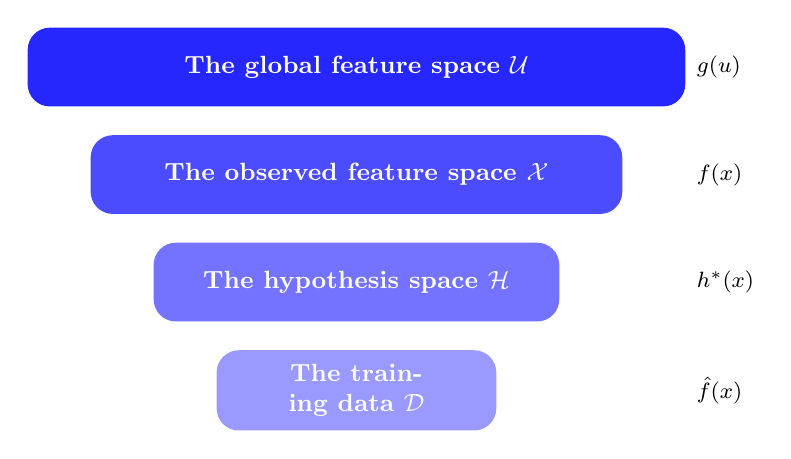
\begin{tikzpicture}[
		% Style des blocs du funnel (largeurs légèrement réduites)
		stage/.style={
			fill=#1,
			draw=none, 
			rounded corners=8pt, 
			text=white, 
			font=\small\bfseries,
			align=center,
			minimum height=1.0cm,
			inner sep=5pt,
		},
		% Style des étiquettes à droite
		labelstyle/.style={
			font=\footnotesize,
			text=black,
			anchor=west
		}
		]
		% --- DÉFINITION DES BLOCS ---
		% Largeurs ajustées : 8cm / 6.4cm / 4.8cm / 3.2cm
		\node[stage=blue!85, text width=8cm] (s1) at (0,0) {The global \mbox{feature} space $\mathcal{U}$};
		
		\node[stage=blue!70, text width=6.4cm, below=10pt of s1] (s2) {The observed \mbox{feature} space $\mathcal{X}$};
		
		\node[stage=blue!55, text width=4.8cm, below=10pt of s2] (s3) {The hypothesis space $\mathcal{H}$};
		
		\node[stage=blue!40, text width=3.2cm, below=10pt of s3] (s4) {The training \mbox{data} $\mathcal{D}$};
		
		% --- COORDONNÉES D'ALIGNEMENT ---
		% L décalé à -4.4 pour coller au bloc de 8cm
		% R décalé à 4.2 pour ne pas sortir de la slide
		\coordinate (L) at (-4.4,0); 
		\coordinate (R) at (4.2,0);  
		
		% --- COMMENTS ON THE RIGHT ---
		\node[labelstyle] at (R |- s1) {$g(u)$};
		\node[labelstyle] at (R |- s2) {$f(x)$};
		\node[labelstyle] at (R |- s3) {$h^*(x)$};
		\node[labelstyle] at (R |- s4) {$\hat{f}(x)$};
		
	\end{tikzpicture}
\end{frame}

\begin{frame}{Hierarchy of Learning Spaces}
	We want to predict a car's speed based on its instantaneous fuel consumption:
	\pause
	\begin{itemize}
		\item Instantaneous consumption is indeed an explanatory feature of speed.
		\pause
		\item However, there are other unobserved features that are also relevant: vehicle weight, wind, slope... The true function $f$ will therefore be a highly approximate model of reality $g$.
		\pause
		\item The hypothesis space $\mathcal{H}$ restricts the candidate functions explored, which can introduce additional losses compared to the true function $f$.
		\pause
		\item Finally, we only have a limited set of training data $\mathcal{D}$. The best we can do is obtain an approximation of $h^{*}$, denoted as $\hat{f}$.
	\end{itemize}
\end{frame}

\begin{frame}{Hypothesis Space and Learning Space Hierarchy}
	In summary:
	\begin{itemize}
		\item We denote by $g$ the \textbf{generative process} linking global features to outputs.
		\item We denote by $f$ the \textbf{true} function linking space $\mathcal{X}$ to space $\mathcal{Y}$.
		\item We denote by $h^*$ the \textbf{best} function in the hypothesis space $\mathcal{H}$ linking these same spaces.
		\item We denote by $\hat{f} \in \mathcal{H}$ the \textbf{estimation} of $f$ after training the algorithm on data $\mathcal{D}$.
	\end{itemize}
\end{frame}

\subsection[Supervised Learning]{Supervised Learning}

\begin{frame}{Supervised Learning}
	\begin{block}{Supervised Learning Formulation}
		The objective of supervised learning is to find a function $\hat{f}: \mathcal{X} \to \mathcal{Y}$ within the hypothesis space $\mathcal{H}$ that serves as a good \textbf{estimator} of the \textbf{true} function $f$, using the data $\mathcal{D} = \begin{Bmatrix}(x^{(i)}, y^{(i)})\end{Bmatrix}_{i=1}^n$:
		\begin{equation*}
			y = f(x) + \epsilon
		\end{equation*}
		Where $\epsilon$ represents an uncertainty linked to measurement noise in the observed data or to unobserved explanatory variables.
		\hfill
	\end{block}
	\vspace{0.5cm}
	\pause
	We denote by $\hat{y} = \hat{f}(x)$ the prediction made by the model for an input $x$. \\
	\vspace{0.5cm}
	\pause
	A good estimator $\hat{f}$ is one that minimizes a \textbf{loss function} $L(y, \hat{y})$ over the set of observed data $\mathcal{D}$, also called training data.
\end{frame}

\begin{frame}{Regression Problem}
	\begin{block}{Regression Problem Setting}
		In a \textbf{regression} problem, the output variable is quantitative: $\mathcal{Y} \subseteq \mathbb{R}$. \\
		\vspace{0.3cm}
		The loss function $L$ measures a distance between the algorithm's prediction $\hat{y}$ and the observed value $y$. 
	\end{block}
	\pause
	An example of a loss function is the squared error:
	\begin{equation}
		L(y, \hat{y}) = \left( y - \hat{y}\right)^2
		\nonumber
	\end{equation}
\end{frame}

\begin{frame}{Classification Problem}
	\begin{block}{Binary Classification Problem Setting}
		In a \textbf{binary classification} problem, the output variable is qualitative: $\mathcal{Y} = \{0, 1\}$. \\
		\vspace{0.3cm}
		The loss function $L$ acts as a counter for classification errors. \\
		\vspace{0.3cm}
	\end{block}
	\pause
	An example of a loss function would be the 0-1 loss function:
	\begin{equation}
		\begin{cases}
			L(y, \hat{y}) = 0 & \text{si } y = \hat{y} \\
			L(y, \hat{y}) = 1 & \text{si } y \ne \hat{y}
		\end{cases}
		\nonumber
	\end{equation}
	\pause
	\begin{itemize}
		\item \textbf{Note on uncertainty:} Here, $\epsilon = y - f(x)$ represents a discrete uncertainty taking its values in $\{-1, 0, 1\}$.
		\item \textbf{Note on optimization:} The 0-1 function is non-differentiable. In practice, we will use surrogates (such as log-likelihood).
	\end{itemize}
	
\end{frame}
\section[Linear Models]{Linear Models}

\begin{frame}{Linear Models}
	In this section, we will study 2 linear models for regression and classification problems:
	\begin{itemize}
		\item \textbf{Linear regression} for regression problems.
		\item \textbf{Logistic regression} for classification problems.
	\end{itemize}
\end{frame}

\subsection[Linear Regression]{Linear Regression}

\begin{frame}{Linear Regression}
	\begin{columns}
		\begin{column}{0.5\textwidth}
			\begin{figure}
				\centering
				\includegraphics[height=0.8\linewidth]{Images/regression_lineaire_3}
				\label{fig:regression-lineaire-3}
			\end{figure}			
		\end{column}
		\begin{column}{0.5\textwidth}
			\begin{table}
				\centering
				\begin{tabular}{|c|c|}
					\hline
					\textbf{Height} (cm) & \textbf{Weight} (kg) \\ \hline
					190              & 112 \\
					172              & 85  \\
					186              & 135 \\
					180              & 92  \\
					\hline
				\end{tabular}
			\end{table}
		\end{column}
	\end{columns}
\end{frame}

\begin{frame}{Examples}
	\begin{columns}
		\begin{column}{0.5\textwidth}
			\begin{figure}
				\centering
				\includegraphics[height=0.8\linewidth]{Images/regression_lineaire_1}
				\label{fig:regression-lineaire-1}
			\end{figure}
		\end{column}
		\begin{column}{0.5\textwidth}
			\begin{figure}
				\centering
				\includegraphics[height=0.8\linewidth]{Images/regression_lineaire_2}
				\label{fig:regression-lineaire-2}
			\end{figure}
		\end{column}		
	\end{columns}
	\pause
	The idea is to construct a straight line that passes as close as possible to the observations $\mathcal{D}$. The algorithm attempts to minimize the total distance between the observations and the predictions.
\end{frame}

\begin{frame}{Model}
	The linear regression model can be written in a simple form:
	\begin{equation}
		\text{weight}^{(i)} \approx \beta_0 + \beta_1 \times \text{height}^{(i)}
		\nonumber
	\end{equation}
	An equivalent vector form would be:
	\begin{equation}
		\text{weight}^{(i)} \approx \begin{pmatrix}1 & \text{height}^{(i)}\end{pmatrix} \begin{pmatrix}\beta_0 \\ \beta_1\end{pmatrix}
		\nonumber
	\end{equation}	
\end{frame}

\begin{frame}{Model}
	The advantage of this vector form is that it can scale into a matrix form, allowing us to make multiple predictions at once by stacking:
	\begin{equation}
		\begin{pmatrix}\text{weight}^{(1)} \\ \text{weight}^{(2)} \\ \text{weight}^{(3)} \\ \text{weight}^{(4)}\end{pmatrix} \approx \begin{pmatrix}1 & \text{height}^{(1)} \\ 1 & \text{height}^{(2)} \\ 1 & \text{height}^{(3)} \\ 1 & \text{height}^{(4)} \end{pmatrix} \begin{pmatrix}\beta_0 \\ \beta_1\end{pmatrix}
		\nonumber
	\end{equation}
	\pause
	And in a more condensed form:
	\begin{equation}
		Y \approx \tilde{X} \beta
		\nonumber
	\end{equation}
\end{frame}

\begin{frame}{Formulation}
	Let $\mathcal{X} \subseteq \mathbb{R}^d$ be the input feature space, $\mathcal{Y} \subseteq \mathbb{R}$ the output feature space, and $\mathcal{D} = \begin{Bmatrix}(x^{(i)}, y^{(i)})\end{Bmatrix}_{i=1}^n$ the training data. We define the mapping $\Phi$ that performs the transition to the augmented space $\tilde{\mathcal{X}} \subseteq \mathbb{R}^{d+1}$:
	\begin{equation}
		\begin{aligned}
			\Phi: \mathcal{X} &\to \tilde{\mathcal{X}} \\
			x^{(i)} &\mapsto \tilde{x}^{(i)} = \begin{pmatrix}1 & x^{(i)}\end{pmatrix}
			\nonumber
		\end{aligned}
	\end{equation}
	The hypothesis space $\mathcal{H}: \mathcal{X} \to \mathcal{Y}$ in the context of linear regression is:
	\begin{equation}
		\mathcal{H} = \begin{Bmatrix}h: x \mapsto \Phi(x) \beta \mid \beta \in \mathbb{R}^{d+1}\end{Bmatrix}
		\nonumber
	\end{equation}
\end{frame}

\begin{frame}{Matrix Stacking}
	For the training data $\mathcal{D}$, a design matrix $\tilde{X}$ is constructed by vertically stacking the augmented observations $\tilde{x}^{(i)}$:
	\begin{equation}
		\tilde{X} = \begin{pmatrix}\tilde{x}^{(1)} \\ \tilde{x}^{(2)} \\ \vdots \\ \tilde{x}^{(n)} \end{pmatrix} \in \mathcal{M}_{n, d+1}(\mathbb{R})
		\nonumber
	\end{equation}
	We denote by $Y$ the vertical stack of the observed output features:
	\begin{equation}
		Y = \begin{pmatrix}y^{(1)} \\ y^{(2)} \\ \vdots \\ y^{(n)} \end{pmatrix} \in \mathcal{M}_{n, 1}(\mathbb{R})
		\nonumber
	\end{equation}	
\end{frame}

\begin{frame}{Method of Least Squares}
	The method of least squares seeks to minimize the sum of squared errors:
	\begin{equation}
		\begin{aligned}
			J(\beta) &= \sum_{i=1}^n \left(y^{(i)} - \tilde{x}^{(i)} \beta\right)^2 \\
			&= \left(Y - \tilde{X} \beta\right)^T \left(Y - \tilde{X} \beta\right)
		\end{aligned}
		\nonumber
	\end{equation}
	$\hat{\beta}$ is an estimator of $\beta$ that minimizes this sum of squared errors:
	\begin{equation}
		\hat{\beta} = \underset{\beta \in \mathbb{R}^{d+1}}{\text{arg min}}\left(\left(Y - \tilde{X} \beta\right)^T \left(Y - \tilde{X} \beta\right)\right)
		\nonumber
	\end{equation}
\end{frame}

\begin{frame}{Method of Least Squares}
	An analytical solution exists for this optimization problem:
	\begin{equation}
		\begin{aligned}
			&\hat{\beta} = \left( \tilde{X}^T \tilde{X}\right)^{-1} \tilde{X}^T Y \\
			&\hat{\beta} \in \mathcal{M}_{d+1, 1}(\mathbb{R}) \\
			\nonumber
		\end{aligned}
	\end{equation}
	To exist, this solution requires the matrix $\left(\tilde{X}^T \tilde{X}\right)$ to be invertible. This means that the columns of $\tilde{X}$ must be linearly independent.
	The estimation function $\hat{f}$ is therefore:
	\begin{equation}
		\begin{aligned}
			\hat{f}: \mathcal{X} &\to \mathcal{Y} \\
			x &\mapsto \Phi(x) \hat{\beta}
			\nonumber
		\end{aligned}
	\end{equation}
\end{frame}

\begin{frame}{Assumptions of the Method of Least Squares}
	The method of least squares relies on a certain number of assumptions regarding the uncertainty $\epsilon$ in order to derive the covariance matrix of $\hat{\beta}$. As a reminder, in supervised learning we seek a function estimating the true function $f$ defined as:
	\begin{equation}
		y = f(x) + \epsilon
		\nonumber
	\end{equation}
	Let $X$ be the matrix stack of the observed input features. $\epsilon$ must satisfy the following conditions:
	\begin{itemize}
		\item The \textbf{exogeneity} condition: $\mathbb{E}[\epsilon \mid X] = 0$.
		\begin{itemize}
			\item This condition guarantees that $\mathbb{E}[\hat{\beta}] = \beta$. Here, $\beta$ is the one from $h^*$.
			\item There is no functional link between the expectation of $\epsilon$ and the input data.
		\end{itemize}
		\item The \textbf{homoscedasticity} condition: $\text{Var}[\epsilon \mid X] = \sigma_{\epsilon}^2$.
		\begin{itemize}
			\item There is no functional link between the variance of $\epsilon$ and the input data.
		\end{itemize}
		\item The \textbf{independence} condition implies: $\text{Cov}[\epsilon^{(i)}, \epsilon^{(j)}] =0 \quad \forall i \ne j$
	\end{itemize}
\end{frame}

\begin{frame}{Learning Space Hierarchy and Linear Regression}
	\begin{columns}
		\begin{column}{0.4\textwidth}
			\begin{figure}
				\centering
				\includegraphics[width=1.0\linewidth]{Images/regression_lineaire}
				\label{fig:poids-taille}
			\end{figure}			
		\end{column}
		\begin{column}{0.6\textwidth}
			The linear model is far from perfect:
			\begin{itemize}
				\item Either the linearity assumption is incorrect. The hypothesis space $\mathcal{H}$ is not the most appropriate.
				\item Or some features are missing, such as density, hip circumference, muscle-to-fat mass ratio...
				\item Or there is significant measurement noise in the height and/or weight.
				\item Or any combination of the elements above!
			\end{itemize}
		\end{column}
	\end{columns}
\end{frame}	

\begin{frame}{Hypothesis Spaces and Linear Regression}
	It would have been possible to consider another mapping $\Phi'$ to transition from the input space $\mathcal{X} \subseteq \mathbb{R}$ to the augmented space $\tilde{\mathcal{X}}' \subseteq \mathbb{R}^3$, for example:
	\begin{equation}
		\begin{aligned}
			\Phi': \mathcal{X} &\rightarrow \tilde{\mathcal{X}}' \\
			x^{(i)} &\mapsto \tilde{x}^{(i)} = \begin{pmatrix}1 & x^{(i)} & \left(x^{(i)}\right)^2\end{pmatrix}
			\nonumber
		\end{aligned}		
	\end{equation}
	The linear regression effectively becomes a degree-2 polynomial regression. Thus, a new hypothesis space $\mathcal{H}'$ is explored:
	\begin{equation}
		\mathcal{H}' = \begin{Bmatrix}h: x \mapsto \Phi'(x) \beta \mid \beta \in \mathbb{R}^3\end{Bmatrix}
		\nonumber
	\end{equation}	
\end{frame}

\begin{frame}{Hypothesis Spaces and Linear Regression}
	Within the context of linear regression, the nature of the mapping $\Phi$ is a \textbf{hyperparameter} of the machine learning algorithm. \\
	\vspace{0.5cm}
	The coefficients $\beta$ of the polynomial are the \textbf{parameters} of the algorithm. These are the parameters explored by the hypothesis space $\mathcal{H}$.\\
	\vspace{0.5cm}
	The method of least squares provides an estimation $\hat{f}$ of the true function $f$ among the functions $h$ in space $\mathcal{H}$.
\end{frame}

\subsection[Logistic Regression]{Logistic Regression}

\begin{frame}{Logistic Regression}
	\begin{table}
		\centering
		\begin{tabular}{|c|c|}
			\hline
			\textbf{Weight} (kg) & \textbf{Position} \\ \hline
			112 &  forward = 1       \\
			85  &  back = 0 \\
			135 &  forward = 1       \\
			92  &  back = 0 \\
			\hline
		\end{tabular}
	\end{table}
	\begin{figure}
		\centering
		\includegraphics[width=0.9\linewidth]{Images/regression_logistique_1}
		\label{fig:regression-logistique-1}
	\end{figure}			
\end{frame}

\begin{frame}{Logistic Function}
	\begin{columns}
		\begin{column}{0.6\textwidth}
			\begin{figure}
				\centering
				\includegraphics[width=1.0\linewidth]{Images/regression_logistique_3}
				\label{fig:regression-logistique-3}
			\end{figure}			
		\end{column}
		\begin{column}{0.4\textwidth}
			\begin{equation}
				\begin{aligned}
					\sigma: \mathbb{R} &\to ]0, 1[ \\
					t &\mapsto \frac{1}{1 + e^{-t}}
				\end{aligned}
				\nonumber
			\end{equation}
			\pause
			The idea is to map the forwards to the upper plateau of this function ($\sigma(t) = 1$) and to map the backs to the lower plateau ($\sigma(t) = 0$).
		\end{column}
	\end{columns}
\end{frame}

\begin{frame}{Examples}
	\begin{columns}
		\begin{column}{0.5\textwidth}
			\begin{figure}
				\centering
				\includegraphics[height=0.8\linewidth]{Images/regression_logistique_4}
				\label{fig:regression-logistique-4}
			\end{figure}
		\end{column}
		\begin{column}{0.5\textwidth}
			\begin{figure}
				\centering
				\includegraphics[height=0.8\linewidth]{Images/regression_logistique_5}
				\label{fig:regression-logistique-5}
			\end{figure}
		\end{column}		
	\end{columns}
	\pause
	This logistic regression actually calculates a probability $p$, specifically the probability that a player of a given weight is a forward.
\end{frame}

\begin{frame}{Model}
	The logistic regression model can be written in a relatively simple form:
	\begin{equation}
		p^{(i)} \approx \frac{1}{1 + e^{\displaystyle -\left(\beta_0 + \beta_1 \times \text{weight}^{(i)} \right)}}
		\nonumber
	\end{equation}
	It can be viewed as a linear model inside the exponential, combined with a function that maps the outputs into the probability space $]0, 1[$. \\
\end{frame}

\begin{frame}{Model}
	And in matrix notation:
	\begin{equation}
		p \approx \frac{1}{1 + e^{\displaystyle -\tilde{X} \beta}}
		\nonumber
	\end{equation} \\
	\vspace{0.5cm}
	Condensing it using the logistic function $\sigma$:
	\begin{equation}
		p \approx \sigma\left(\tilde{X} \beta\right)
		\nonumber
	\end{equation}
\end{frame}

\begin{frame}{Formulation}
	Let $\mathcal{X} \subseteq \mathbb{R}^d$ be the input feature space, $\mathcal{Y} = \{0, 1\}$ the output feature space, and $\mathcal{D} = \begin{Bmatrix}(x^{(i)}, y^{(i)})\end{Bmatrix}_{i=1}^n$ the training data. We define the mapping $\Phi$ that performs the transition to the augmented space $\tilde{\mathcal{X}} \subseteq \mathbb{R}^{d+1}$:
	\begin{equation}
		\begin{aligned}
			\Phi: \mathcal{X} &\to \tilde{\mathcal{X}} \\
			x^{(i)} &\mapsto \tilde{x}^{(i)} = \begin{pmatrix}1 & x^{(i)}\end{pmatrix}
			\nonumber
		\end{aligned}
	\end{equation}
	The hypothesis space $\mathcal{H}: \mathcal{X} \to ]0, 1[$ in the context of logistic regression is:
	\begin{equation}
		\mathcal{H} = \begin{Bmatrix}h: x \mapsto \displaystyle \frac{1}{1 + e^{-\Phi(x) \beta}} \mid \beta \in \mathbb{R}^{d+1}\end{Bmatrix}
		\nonumber
	\end{equation}
\end{frame}

\begin{frame}{Assumptions and Iterative Approach}
	Unlike linear regression, there is no analytical solution to this problem. To determine $\hat{\beta}$, we will therefore need to use an \textbf{iterative} approach. \\
\end{frame}

\begin{frame}{Bernoulli Distribution}
	One approach to solving the problem is to consider each observation $y^{(i)}$ as the realization of a random variable $Y^{(i)}$ following a \textbf{Bernoulli distribution} with parameter $p^{(i)}$. The observations are independent but not identically distributed.\\
	\vspace{0.5cm}
	\pause
	As a reminder, a random variable $Y^{(i)}$ following a Bernoulli distribution with parameter $p^{(i)}$ is such that:
	\begin{equation*}
		\begin{cases}
			P(Y^{(i)} = 1) = p^{(i)} \\
			P(Y^{(i)} = 0) = 1 - p^{(i)}
		\end{cases}
	\end{equation*}
	Or in a condensed form with $y \in \{0, 1\}$:
	\begin{equation*}
		P(Y^{(i)} = y^{(i)}) = \left(p^{(i)}\right)^{y^{(i)}} \left(1 - p^{(i)}\right)^{1 - y^{(i)}}
	\end{equation*}
\end{frame}
	
\begin{frame}{Maximum Likelihood Estimation}
	The likelihood of our sample $\mathcal{D}$ is then:
	\begin{equation}
		\mathcal{L}(\beta) = P(Y = \begin{Bmatrix}y^{(i)}\end{Bmatrix}_{i=1}^n \mid \beta, \tilde{X})
		\nonumber
	\end{equation} \\
	\vspace{0.5cm}
	\pause
	The idea consists in finding $\hat{\beta}$ such that it maximizes the likelihood of the observations:
	\begin{equation}
		\hat{\beta} = \underset{\beta \in \mathbb{R}^{d+1}}{\text{arg max}} \, \mathcal{L}(\beta)
		\nonumber
	\end{equation} \\
	\vspace{0.5cm}
	\pause
	This maximum likelihood method assumes that the exogeneity and independence conditions of $\epsilon^{(i)}$ are satisfied in order to obtain the best possible estimator.
\end{frame}

\begin{frame}{Intuition}
	Let us consider a "forward", to whom we have assigned the value $y^{(i)}=1$. The random variable is $Y^{(i)}$. If the associated Bernoulli distribution is well calibrated, we should have $P(Y^{(i)} = 1)$ very close to 1 and $P(Y^{(i)} = 0)$ very close to 0. \\
	\vspace{0.5cm}
	\pause
	For a "back", to whom we have assigned the value $y^{(i)}=0$, the reverse holds true. We want to have $P(Y^{(i)} = 1)$ very close to 0 and $P(Y^{(i)} = 0)$ very close to 1. \\
	\vspace{0.5cm}
	\pause
	This is equivalent to saying that for a "forward" we want the parameter $p^{(i)}$ of the Bernoulli distribution to be close to 1, and for a back, we want this same parameter to be close to 0. \\
\end{frame}

\begin{frame}{Intuition}
	Since $p^{(i)}$ is the prediction of our logistic regression—meaning the probability that observation $i$ is a forward—maximizing the likelihood of the set of Bernoulli variables amounts to having a well-calibrated logistic regression! \\
	\vspace{0.5cm}
	\pause
	The set of these Bernoulli distributions is actually controlled by a parameter vector $\beta$ that is \textbf{shared} across all distributions. Our problem is therefore over-constrained, just as linear regression was in the previous example.	
\end{frame}

\begin{frame}{Mean Negative Log-Likelihood}
	In practice, it is preferred to minimize a mean negative log-likelihood rather than maximizing a likelihood:
	\begin{equation}
		\hat{\beta} = \underset{\beta \in \mathbb{R}^{d+1}}{\text{arg min}} \, - \frac{1}{n} \ln{\left(\mathcal{L}(\beta)\right)}
		\nonumber
	\end{equation} \\
	\vspace{0.5cm}
	\pause
	Since the observations are independent, this mean negative log-likelihood is in fact:
	\begin{equation}
		- \frac{1}{n}\ln{\left(\mathcal{L}(\beta)\right)} = - \frac{1}{n} \sum_{i=1}^n \ln{\left(P(y^{(i)} \mid \tilde{x}^{(i)}, \beta)\right)}
		\nonumber
	\end{equation}
\end{frame}

\begin{frame}{Mean Cross-Entropy}
	This mean negative log-likelihood takes a very specific and characteristic value. As a reminder, $p^{(i)} = \sigma(\tilde{x}^{(i)} \beta)$:
	\begin{equation}
		\begin{aligned}
			-\frac{1}{n} \ln{\left(\mathcal{L}(\beta)\right)} 
			&= - \frac{1}{n} \sum_{i=1}^n \ln{P(y^{(i)} \mid \tilde{x}^{(i)}, \beta)} \\
			&= - \frac{1}{n} \sum_{i=1}^n \ln{\left(\left(p^{(i)}\right)^{y^{(i)}} \left(1 - p^{(i)}\right)^{1 - y^{(i)}}\right)} \\
			&= - \frac{1}{n} \sum_{i=1}^n y^{(i)} \ln{\left(p^{(i)}\right)} + (1 - y^{(i)}) \ln{\left(1 - p^{(i)}\right)}
		\end{aligned}
		\nonumber
	\end{equation}
	This quantity is called the \textbf{mean cross-entropy}!
\end{frame}

\begin{frame}{Cross-Entropy Gradient}
	It can be shown that the derivative of the mean negative log-likelihood with respect to $\beta$ is written as:
	\begin{equation}
		\begin{aligned}
			\nabla_{\beta}\left(- \frac{1}{n} \ln{\left(\mathcal{L}(\beta)\right)}\right) 
			&= - \frac{1}{n} \sum_{i=1}^n \left(y^{(i)} - \sigma(\tilde{x}^{(i)} \beta)\right) \tilde{x}^{(i)T} \\
			&= - \frac{1}{n} \tilde{X}^T \left(Y - \sigma\left(\tilde{X} \beta\right)\right)
		\end{aligned}
		\nonumber
	\end{equation}
	This gradient brings forward 2 terms:
	\begin{itemize}
		\item $\left(Y - \sigma\left(\tilde{X} \beta\right)\right)$ which is the difference between the probability associated with the observed value and the probability predicted by the logistic regression for a given parameter vector $\beta$.
		\item $\tilde{X}^T$ which represents simply the observed (and augmented) input features.
	\end{itemize}
\end{frame}

\begin{frame}{Gradient Descent}
	The minimization of the mean negative log-likelihood can be performed using a gradient descent method. The function to minimize is strictly convex (provided the columns of $\tilde{X}$ are linearly independent). Thus, gradient descent is guaranteed to find a \textbf{global} minimum. \\
	\vspace{0.5cm}
	We denote by $\alpha \in \mathbb{R}^+$ the learning rate. A value that is too large can lead to numerical instability in the gradient descent, while a value that is too small can result in overly slow convergence. A value of $\alpha = 0.001$ is typical to start with. \\
	\vspace{0.5cm}
	We denote by $\epsilon \in \mathbb{R}^+$ the tolerance threshold to stop the gradient descent, for example $\epsilon = 10^{-6}$.
\end{frame}

\begin{frame}{Gradient Descent}
	The gradient descent algorithm can be described as follows:
	\begin{enumerate}
		\item Set an initial value of $\hat{\beta}_{k=0} = 0_{d+1}$
		\item Loop until convergence:
		\begin{itemize}
			\item Compute the $n$ probabilities $p_k = \sigma(\tilde{X} \beta_{k})$
			\item Compute the gradient $\nabla_{\beta}\left(- \frac{1}{n} \ln{\mathcal{L}(\beta)}\right)$
			\item Compute the increment of $\hat{\beta}$: $\delta_k = - \alpha \nabla_{\beta}\left(- \frac{1}{n} \ln{\mathcal{L}(\beta)}\right)$
			\item Update $\hat{\beta}$: $\hat{\beta}_{k+1} \leftarrow \hat{\beta}_{k} + \delta_k$
			\item Compute the squared Euclidean norm $\|\delta_k \|_2^2$
			\item If $\|\delta_k \|_2^2 < \epsilon$, then convergence is reached.
		\end{itemize}
	\end{enumerate}
\end{frame}

\subsection[Summary]{Summary}

\begin{frame}{Summary: Linear vs Logistic}
	\begin{table}
		\renewcommand{\arraystretch}{1.5} % Pour aérer le tableau
		\begin{tabular}{|l|c|c|}
			\hline
			\textbf{Property} & \textbf{Linear Regression} & \textbf{Logistic Regression} \\ \hline
			\textbf{Nature of $Y$} & Continuous ($\mathbb{R}$) & Discrete ($\{0, 1\}$) \\ \hline
			\textbf{Model} & $y \approx \tilde{X}\beta$ & $p \approx \sigma(\tilde{X}\beta)$ \\ \hline
			\textbf{Loss Function} & Squared Error & Cross-Entropy \\ \hline
			\textbf{Objective} & Minimize & Minimize \\ \hline
			\textbf{Resolution} & \textbf{Analytical} (direct) & \textbf{Numerical} (iterative) \\ \hline
			\textbf{Solution} & $\hat{\beta} = (\tilde{X}^T\tilde{X})^{-1}\tilde{X}^TY$ & Gradient descent \\ \hline
		\end{tabular}
	\end{table}
	Note: For a classification problem, minimizing Cross-Entropy is equivalent to maximizing Log-Likelihood. For a regression problem, under the condition where the uncertainty $\epsilon$ is Gaussian, minimizing the mean squared error is equivalent to maximizing the Log-Likelihood.
\end{frame}
\section[Model Selection and Validation]{Model Selection and Validation}

\begin{frame}{Model Selection and Validation}
	In this section, we will discuss model selection and validation for a supervised learning problem: \\
	\vspace{0.5cm}
	\begin{itemize}
		\item \textbf{Selection}: which model is the best among several hypothesis spaces?
		\item \textbf{Validation}: how can we ensure that our model achieves sufficient performance?
	\end{itemize}
\end{frame}

\subsection{Error Decomposition}

\begin{frame}{Error Decomposition}
	To better understand how to perform model selection and validation, we need to spend some more time on a model's \textbf{error decomposition}.
\end{frame}

\begin{frame}{Empirical Risk}
	Minimizing the loss function $L$ over the training data $\mathcal{D}$ is equivalent to minimizing the \textbf{empirical} risk defined as follows:
	\begin{block}{Definition: Empirical Risk}
		The empirical risk is a function $R_n: \mathcal{H} \to \mathbb{R}^+$ that measures the performance of any hypothesis $h \in \mathcal{H}$ on the training data $\mathcal{D}$:
		\begin{equation}
			R_n = \frac{1}{n} \sum_{i=1}^n L\left(y^{(i)}, h\left(x^{(i)}\right)\right)
			\nonumber
		\end{equation}
		\hfill
	\end{block}
\end{frame}

\begin{frame}{Empirical Risk}
	Training the supervised algorithm yields the estimator $\hat{f}$ that minimizes the empirical risk from the data $\mathcal{D}$:
	\begin{equation}
		\hat{f} = \underset{h \in \mathcal{H}}{\text{arg min  }}R_n(h)
		\nonumber
	\end{equation}
\end{frame}

\begin{frame}{Empirical Risk for Linear Regression}
	In the case of linear regression, the loss function is the squared error function. Searching for an estimator $\hat{f}$ therefore corresponds to minimizing:
	\begin{equation}
		\hat{f} = \underset{h \in \mathcal{H}}{\text{arg min  }} \frac{1}{n} \sum_{i=1}^n \left( y^{(i)} - \hat{y}^{(i)}\right)^2
		\nonumber
	\end{equation}
	Which is equivalent to what the least squares algorithm achieves (up to a factor of $1/n$).
\end{frame}

\begin{frame}{Empirical Risk for Logistic Regression}
	In the case of logistic regression, the loss function is the mean cross-entropy (mean negative log-likelihood). Searching for an estimator $\hat{f}$ therefore corresponds to minimizing:
	\begin{equation}
		\hat{f} = \underset{h \in \mathcal{H}}{\text{arg min  }} - \frac{1}{n} \sum_{i=1}^n y^{(i)} \ln{\left(p^{(i)}\right)} + (1 - y^{(i)}) \ln{\left(1 - p^{(i)}\right)}
		\nonumber
	\end{equation}
	This is the quantity we minimized earlier using gradient descent.
\end{frame}

\begin{frame}{Model and Hypothesis Comparison}
	Let us return to the linear regression problem of predicting a player's weight from their height, and consider two hypothesis spaces:
	\begin{itemize}
		\item $\mathcal{H}_1$: the hypothesis space for univariate polynomials of degree 1.
		\item $\mathcal{H}_3$: the hypothesis space for univariate polynomials of degree 3.
	\end{itemize}
\end{frame}

\begin{frame}{Which Model Is Better? Or Which Hypothesis?}
	\begin{columns}
		\begin{column}{0.5\textwidth}
			\begin{figure}
				\centering
				\includegraphics[height=0.8\linewidth]{Images/comparaison_modeles_1}
				\label{fig:comparaison-modeles-1}
			\end{figure}
		\end{column}
		\begin{column}{0.5\textwidth}
			\begin{figure}
				\centering
				\includegraphics[height=0.8\linewidth]{Images/comparaison_modeles_2}
				\label{fig:comparaison-modeles-2}
			\end{figure}
		\end{column}		
	\end{columns}
\end{frame}

\begin{frame}{Which Model Is Better? Or Which Hypothesis?}
	\begin{itemize}
		\item For a linear regression, we seek to minimize the squared error...
		\pause
		\item ...but this is not the \textbf{goal}, it is a \textbf{means to an end}. The goal is to find a \textbf{relationship} between the input and output features that is as close as possible to the true function $f(x)$ and the generative process $g(u)$.
		\pause
		\item For the hypothesis space $\mathcal{H}_1$, $\hat{\beta}_0$ has no tangible interpretation: a player who is 0 cm tall would weigh -291 kg? On the other hand, $\hat{\beta}_1$ informs us that for each additional 1 cm, the weight increases on average by 2 kg. This does not seem absurd.
		\pause
		\item For the hypothesis space $\mathcal{H}_3$, the model shows that weight is lost up to 175 cm, then gained up to 185 cm, before losing weight again beyond 185 cm. This seems highly implausible!
	\end{itemize}
\end{frame}

\begin{frame}{Which Model Is Better? Or Which Hypothesis?}
	\begin{itemize}
		\item Hypothesis $\mathcal{H}_1$ is better here.
		\pause
		\item Our \textbf{a priori knowledge} of the problem allows us to distinguish the better hypothesis. What should we do when we have no a priori knowledge?
		\pause
		\item We consult with domain \textbf{experts}.
		\pause
		\item But can we really do \textit{nothing} with mathematics?
		\pause
		\item \textit{Yes}, we can! (though this does not dispense with surrounding oneself with domain experts).
	\end{itemize}
\end{frame}

\begin{frame}{Which Model Is Better? Or Which Hypothesis?}
	What is happening with our hypothesis $\mathcal{H}_3$?
	\begin{itemize}
		\item It is likely that we do not have access to all the explanatory variables in our data. Therefore, it is impossible to obtain a model that correctly explains the problem.
		\pause
		\item Yet this is the assumption made when working with $\mathcal{H}_3$. The model has the \textbf{capacity} to fully explain weight using height, giving it a disproportionate amount of importance compared to its actual relevance.
		\pause
		\item This is what we call \textbf{overfitting}: too much importance is placed on certain observed variables.
		\pause
		\item We also say that the model derived from $\mathcal{H}_3$ does not \textbf{generalize} correctly: the rule \textbf{induced} during training does not match reality.
	\end{itemize}
\end{frame}

\begin{frame}{Which Model Is Better? Or Which Hypothesis?}
	\begin{columns}
		\begin{column}{0.5\textwidth}
			\begin{figure}
				\centering
				\includegraphics[height=0.8\linewidth]{Images/comparaison_modeles_3}
				\label{fig:comparaison-modeles-3}
			\end{figure}
		\end{column}
		\begin{column}{0.5\textwidth}
			\begin{figure}
				\centering
				\includegraphics[height=0.8\linewidth]{Images/comparaison_modeles_4}
				\label{fig:comparaison-modeles-4}
			\end{figure}
		\end{column}		
	\end{columns}
\end{frame}

\begin{frame}{Which Model Is Better? Or Which Hypothesis?}
	In the previous example, when using a larger dataset:
	\begin{itemize}
		\item The degree-3 polynomial now appears monotonic but remains implausible.
		\item The straight line exhibits a slope $\hat{\beta}_1$ that differs from the previous model. 
	\end{itemize}
	\pause
	\vspace{0.5cm}
	Overfitting is not solely a consequence of a model complexity (or capacity) being too high, but rather a consequence of the ratio between model complexity and the amount of training data observed. \\
	\vspace{0.5cm}
	The trained model $\hat{f}$ \textbf{varies} with different sets of training data $\mathcal{D}$.
	\pause
\end{frame}

\begin{frame}{Which Model Is Better? Or Which Hypothesis?}
	What can we do as mathematicians?
	\begin{itemize}
		\item We must provide a \textbf{counterweight} to the empirical risk.
		\pause
		\item This counterweight is a new metric: the \textbf{true risk}.
		\pause
		\item The idea, quite simple, is to \textbf{verify} the model with observations that were not used during training and to \textbf{evaluate} this metric on this \textbf{test sample}. 
	\end{itemize}
\end{frame}

\begin{frame}{True Risk}
	The \textbf{true} risk generalizes the notion of empirical risk to the spaces $\mathcal{X}$ and $\mathcal{Y}$:
	\begin{block}{Definition: True Risk}
		The true risk is a function $R: \mathcal{H} \to \mathbb{R}^+$ that measures the performance of any hypothesis $h$ over the spaces $\mathcal{X}$ and $\mathcal{Y}$:
		\begin{equation}
			R = \mathbb{E}_{(\mathcal{X}, \mathcal{Y}) \sim \mathcal{P}}\left[L\left(y^{(i)}, h\left(x^{(i)}\right)\right)\right]
			\nonumber
		\end{equation}
		\hfill
	\end{block}
	\pause
	Instead of averaging the loss function over the explored data, the true risk averages the loss function over the complete set of all possible observations. \\
	\pause
	In practice, it is difficult or even impossible to compute the true risk. We can obtain an estimation using a \textbf{test sample}.
\end{frame}

\begin{frame}{Generalization Gap}
	\begin{block}{Definition: Generalization Gap}
		The generalization gap is a function $\mathcal{H} \to \mathbb{R}$ that measures the difference between the true risk and the empirical risk:
		\begin{equation*}
			\text{Gap} = R - R_n
		\end{equation*}
		\hfill
	\end{block}
	\pause
	A positive generalization gap means that the algorithm performs worse on its application space than on the space on which it was trained. This is a sign of overfitting, or a failure of the algorithm to generalize.
\end{frame}
	
\begin{frame}{Pointwise True Risk}
	\begin{block}{Definition: Pointwise True Risk}
		The \textbf{pointwise true risk} is a function $R_{xy}: \mathcal{H} \to \mathbb{R}^+$ that measures the performance of any hypothesis $h$ at \textbf{a single point} of the spaces $\mathcal{X}$ and $\mathcal{Y}$ while considering \textbf{multiple} training datasets:
		\begin{equation*}
			R_{xy} = \mathbb{E}_{\mathcal{D}}\left[L\left(y^{(i)}, h\left(x^{(i)}\right)\right)\right]
		\end{equation*}
			\hfill
	\end{block}
	\vspace{0.5cm}
	\pause
	Different datasets can lead to different estimators $h$. It is therefore interesting to see, for a given hypothesis space $\mathcal{H}$, how the estimators $h$ behave \textbf{on average} at a single point of the spaces $\mathcal{X}$ and $\mathcal{Y}$.
\end{frame}
		
\begin{frame}{Bias-Variance Decomposition}
	For a regression problem, using the squared error as the loss function allows the pointwise true risk to be decomposed as follows:
	\begin{equation*}
		R_{xy} = \left(\mathbb{E}_{\mathcal{D}}\left[f(x) - \hat{f}(x)\right]\right)^2 + \mathbb{E}_{\mathcal{D}}\left[\left(\hat{f}(x) - \mathbb{E}_{\mathcal{D}}\left[\hat{f}(x)\right]\right)^2\right] + \sigma_{\epsilon}^2
	\end{equation*}
	This decomposition is called the \textbf{bias-variance decomposition} of the error.
\end{frame}
			
\begin{frame}{Bias-Variance Decomposition}
	\begin{itemize}
		\item $\mathbb{E}_{\mathcal{D}}\left[f(x) - \hat{f}(x)\right]$ is called the \textbf{bias} of the model. This is an approximation error.
		\item $\mathbb{E}_{\mathcal{D}}\left[\left(\hat{f}(x) - \mathbb{E}_{\mathcal{D}}\left[\hat{f}(x)\right]\right)^2\right]$ is called the \textbf{variance} of the model. This is an estimation error.
		\item $\sigma_{\epsilon}^2$ is the variance of the uncertainties on the observed data. This is an \textbf{irreducible} error, called the Bayes error.
	\end{itemize}
	
	\pause
	\vspace{0.5cm}
	
	The model has a low pointwise risk, provided it has both low bias and low variance. \\
	The bias measures the average difference between the model and the true function. The variance measures how much the model's prediction changes when the training data changes.
\end{frame}
			
\begin{frame}{Bias-Variance Decomposition}
	Example of bias and variance decomposition. Multiple models are built from different training datasets. A 95\% confidence interval is used to illustrate the variance:
	\begin{columns}
		\begin{column}{0.5\textwidth}
			\begin{figure}
				\centering
				\includegraphics[height=0.8\linewidth]{Images/biais_variance_1}
				\label{fig:biais-variance-1}
			\end{figure}
		\end{column}
		\begin{column}{0.5\textwidth}
			\begin{figure}
				\centering
				\includegraphics[height=0.8\linewidth]{Images/biais_variance_2}
				\label{fig:biais-variance-2}
			\end{figure}
		\end{column}		
	\end{columns}
\end{frame}

\begin{frame}[fragile]{Error Decomposition}
	% On utilise hspace pour manger la marge de gauche et recentrer visuellement
	\hspace*{-0.5cm}
	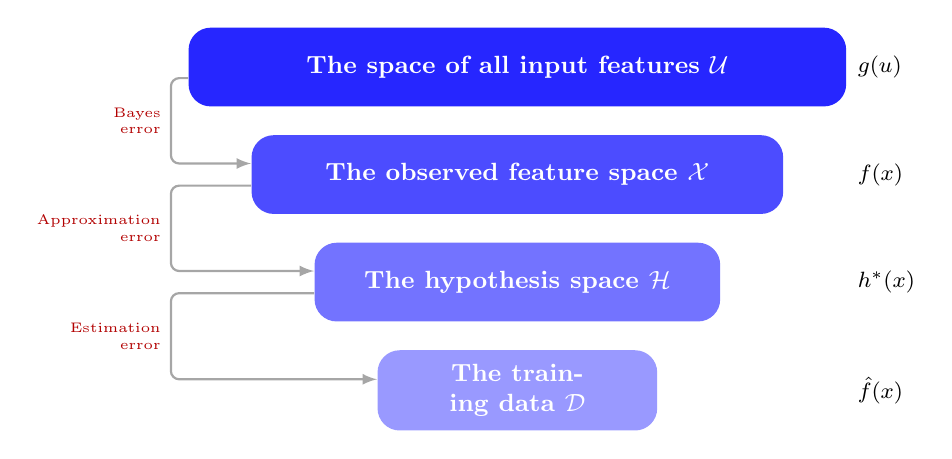
\begin{tikzpicture}[
		% Style des blocs du funnel (largeurs légèrement réduites)
		stage/.style={
			fill=#1,
			draw=none, 
			rounded corners=8pt, 
			text=white, 
			font=\small\bfseries,
			align=center,
			minimum height=1.0cm,
			inner sep=5pt,
		},
		% Style des flèches à gauche
		flowarrow/.style={
			->,
			>=latex,
			thick,
			gray!70,
			rounded corners=3pt
		},
		% Style des étiquettes à droite
		labelstyle/.style={
			font=\footnotesize,
			text=black,
			anchor=west
		}
		]
		% --- DÉFINITION DES BLOCS ---
		% Largeurs ajustées : 8cm / 6.4cm / 4.8cm / 3.2cm
		\node[stage=blue!85, text width=8cm] (s1) at (0,0) {The space of all input \mbox{features} $\mathcal{U}$};
		
		\node[stage=blue!70, text width=6.4cm, below=10pt of s1] (s2) {The observed \mbox{feature} space $\mathcal{X}$};
		
		\node[stage=blue!55, text width=4.8cm, below=10pt of s2] (s3) {The hypothesis space $\mathcal{H}$};
		
		\node[stage=blue!40, text width=3.2cm, below=10pt of s3] (s4) {The training \mbox{data} $\mathcal{D}$};
		
		% --- COORDONNÉES D'ALIGNEMENT ---
		% L décalé à -4.4 pour coller au bloc de 8cm
		% R décalé à 4.2 pour ne pas sortir de la slide
		\coordinate (L) at (-4.4,0); 
		\coordinate (R) at (4.2,0);  
		
		% --- COMMENTS ON THE RIGHT ---
		\node[labelstyle] at (R |- s1) {$g(u)$};
		\node[labelstyle] at (R |- s2) {$f(x)$};
		\node[labelstyle] at (R |- s3) {$h^*(x)$};
		\node[labelstyle] at (R |- s4) {$\hat{f}(x)$};
		
		% --- FLÈCHES À GAUCHE ---
		
		% Flèche 1 -> 2
		\draw[flowarrow] ([yshift=-4pt]s1.west) -- ([yshift=-4pt]s1.west -| L) |- 
		node[pos=0.25, left, font=\tiny, text=red!70!black, align=right] {Bayes\\error} 
		([yshift=4pt]s2.west);
		
		% Flèche 2 -> 3
		\draw[flowarrow] ([yshift=-4pt]s2.west) -- ([yshift=-4pt]s2.west -| L) |- 
		node[pos=0.25, left, font=\tiny, text=red!70!black, align=right] {Approximation\\error} 
		([yshift=4pt]s3.west);
		
		% Flèche 3 -> 4
		\draw[flowarrow] ([yshift=-4pt]s3.west) -- ([yshift=-4pt]s3.west -| L) |- 
		node[pos=0.25, left, font=\tiny, text=red!70!black, align=right] {Estimation\\error} 
		([yshift=4pt]s4.west);
		
	\end{tikzpicture}
\end{frame}

\begin{frame}{Occam's Razor}
	The hypothesis space $\mathcal{H}$ must represent functions that are complex enough (low bias) to capture the relationships between the input and output variables, but not too complex, so as not to allow the algorithm to place excessive importance on certain input variables (low variance). \\
	\vspace{0.5cm}
	The empirical risk must be minimized while maintaining a small generalization gap. \\
	\vspace{0.5cm}
	If two hypothesis spaces lead to models with similar performance, prefer the simpler hypothesis.
\end{frame}

\begin{frame}{Occam's Razor}
	\begin{columns}
		\begin{column}{0.7\textwidth}
			\begin{figure}
				\centering
				\includegraphics[height=0.9\linewidth]{Images/plan_toulouse_2}
				\label{fig:plan-toulouse-2}
			\end{figure}
		\end{column}
		\begin{column}{0.3\textwidth}
			\pause
			Both paths lead to the same destination. The blue path is faster. However, the red path is much easier to explain to a tourist, and the tourist will be less likely to get lost.
		\end{column}		
	\end{columns}	
\end{frame}

\subsection[Performance Metrics]{Performance Metrics}

\begin{frame}{Performance Metrics}
	In this section, we will introduce the essential performance metrics for regression and classification problems. There are many more than what is mentioned here!
\end{frame}

\begin{frame}{Regression Metrics: The Residual}
	The first metric, central to the regression problem, is the \textbf{residual}. Literally, this metric measures what could not be explained by the model—what \textbf{remains} to be explained:
	\begin{block}{Definition: Residual}
		In a regression problem, the \textbf{residual} for an observation $i$ is the difference between the observed output features and those estimated by the model $\hat{f}: \mathcal{X} \to \mathcal{Y}$:
		\begin{equation}
			r^{(i)} = y^{(i)} - \hat{f}(x^{(i)})
			\nonumber
		\end{equation}
	\end{block}
	\pause
	The residual $r$ should not be confused with either the uncertainty $\epsilon^{(i)} = y^{(i)} - f(x^{(i)})$ or the model error $f(x^{(i)}) - \hat{f}(x^{(i)})$, which combines both approximation error and estimation error. Since the uncertainty $\epsilon^{(i)}$ generally cannot be measured, $r^{(i)}$ is the best possible estimate of it.
\end{frame}

\begin{frame}{Regression Metrics: The Coefficient of Determination}
	The coefficient of determination is defined in terms of the residual sum of squares, denoted as $\text{SS}_{\text{res}}$, and the total sum of squares, denoted as $\text{SS}_{\text{tot}}$.
	\begin{block}{Definition: Coefficient of Determination}
		In a regression problem, the \textbf{coefficient of determination} $R^2$ is a metric measuring the fraction of variance explained:
		\begin{equation}
			R^2 = 1 - \frac{\text{SS}_{\text{res}}}{\text{SS}_{\text{tot}}} = 1 - \frac{\sum_{i=1}^n \left(y^{(i)} - \hat{y}^{(i)}\right)^2}{\sum_{i=1}^n \left(y^{(i)} - \bar{y}\right)^2}
			\nonumber
		\end{equation}
	\end{block}
	\pause
	Note: In the context of linear regression, regardless of the augmentation mapping $\Phi$ featuring a constant $\beta_0$, the coefficient of determination is also the square of the Pearson correlation coefficient between the estimated output features $\hat{y}$ and the observed output features $y$.
\end{frame}
			
\begin{frame}{Regression Metrics: The Coefficient of Determination}
	\begin{itemize}
		\item If the model predicts $\bar{y}$ for any input $x$, then $R^2 = 0$.
		\pause
		\item If the model predicts $y^{(i)}$ for the input $x^{(i)}$ for every observation $i$, then $R^2 = 1$.
		\pause
		\item If the residuals $r^{(i)}$ are zero for every observation $i$, then $R^2 = 1$.
		\pause
		\item Warning! A coefficient of determination close to 1 can hide an overfitting problem. Therefore, this metric should be evaluated on both the training data and test data.
	\end{itemize}
\end{frame}

\begin{frame}{Classification Metric: The Confusion Matrix}
	For an $m$-class classification problem ($\mathcal{Y} = \{0, 1, \cdots, m-1\}$), the confusion matrix allows us to \textbf{count} the predictions made by the model relative to the true class for each observation $k$ out of the $n$ observed data points $\mathcal{D}$:
	\begin{block}{Definition: Confusion Matrix}
		In $m$-class classification, the confusion matrix $C \in \mathcal{M}_{m,m}$ is defined as follows, based on the \textbf{true} classes $y^{(k)}$ and the \textbf{predicted} classes $\hat{y}^{(k)}$ for each observation $k$:
		\begin{equation}
			C_{i,j} = \text{card} \left( \{k \in \{1, 2, \cdots, n\}\} \mid y^{(k)} = i \, \text{and} \, \hat{y}^{(k)} = j \right)
			\nonumber
		\end{equation}
	\end{block}
	\pause
	Note: $\text{card}$ is the \textbf{cardinality} operator indicating the number of elements in a set.
\end{frame}

\begin{frame}{Classification Metric: The Confusion Matrix}
	\begin{alertblock}{Lack of a Global Convention for $C$}
		There is no global convention for the layout of the matrix. In the definition provided, true classes are represented by rows and predicted classes by columns (the convention used by \href{https://scikit-learn.org/stable/modules/generated/sklearn.metrics.confusion_matrix.html}{\texttt{sklearn.metrics.confusion\_matrix}}). \\
		\vspace{0.5cm}
		It is always best to specify (or check) the convention used when communicating a confusion matrix. \\
		\vspace{0.5cm}
		The confusion matrix is named for a reason ;)
	\end{alertblock}
\end{frame}

\begin{frame}{Classification Metric: The Confusion Matrix}
	It is much simpler than it appears. Let us illustrate with a binary classification problem ($m = 2$) where we seek to predict the position (forward = 1 or back = 0) of a rugby player:
	\begin{equation}
		C = 
		\begin{bNiceMatrix}[first-row, last-col]
			\text{predicted: back} & \text{predicted: forward} & \\
			\textcolor{blue}{5} & \textcolor{orange}{2} & \text{true: back} \\
			\textcolor{orange}{1} & \textcolor{blue}{7} & \text{true: forward}
		\end{bNiceMatrix}
		\nonumber
	\end{equation}
	\pause
	\begin{itemize}
		\item There are \textcolor{blue}{5} + \textcolor{blue}{7} correct predictions and \textcolor{orange}{1} + \textcolor{orange}{2} incorrect predictions.
		\pause 
		\item A \textcolor{blue}{diagonal} confusion matrix contains only \textcolor{blue}{correct} predictions.
		\pause 
		\item The \textcolor{orange}{erroneous} predictions are found in the \textcolor{orange}{off-diagonal} terms.
		\pause
		\item Since $\text{forward} = 1$, \textcolor{blue}{7} is the number of \textbf{\textcolor{blue}{true} positives} (TP).
		\pause
		\item \textcolor{blue}{5} is the number of \textbf{\textcolor{blue}{true} negatives} (TN), \textcolor{orange}{2} is the number of \textbf{\textcolor{orange}{false} positives} (FP), and \textcolor{orange}{1} is the number of \textbf{\textcolor{orange}{false} negatives} (FN).
	\end{itemize}
\end{frame}

\begin{frame}{Classification Metric: The Confusion Matrix}
	\begin{block}{Definition: TN, FP, FN, TP}
		In the confusion matrix $C$ for a \textbf{binary} classification, for the $n$ observed data points $\mathcal{D}$, the terms of the matrix have the following designations:
		\begin{equation}
			C = 
			\begin{bNiceMatrix}[first-row, last-col]
				\text{predicted: } \{0\} & \text{predicted: } \{1\} & \\
				\text{True negatives (TN)} & \text{False positives (FP)} & \text{true: } \{0\} \\
				\text{False negatives (FN)} & \text{True positives (TP)} & \text{true: } \{1\} \\
			\end{bNiceMatrix}
			\nonumber
		\end{equation}
		These values are \textbf{counters} such that:
		\begin{equation}
			\text{TN} + \text{FN} + \text{FP} + \text{TP} = n
			\nonumber
		\end{equation}
	\end{block}
	\pause
	\textbf{True} means the algorithm made the correct prediction. \textbf{Negative} means the algorithm predicted class \{0\}, whereas positive means the algorithm predicted class \{1\}.
\end{frame}

\begin{frame}{Classification Metric: The Confusion Matrix}
	We often associate \textbf{rates} with the confusion matrix $C$:
	\begin{equation}
		\begin{cases}
			\displaystyle \frac{\text{TP}}{\text{TP} + \text{FP}} & \text{Precision} \\[10pt]
			\displaystyle \frac{\text{TP}}{\text{TP} + \text{FN}} & \text{Recall} \\[10pt]
			\displaystyle \frac{\text{TN}}{\text{TN} + \text{FN}} & \text{Negative predictive value} \\[10pt]
			\displaystyle \frac{\text{TN}}{\text{TN} + \text{FP}} & \text{Specificity}
		\end{cases}
		\nonumber
	\end{equation}
	\pause
	Note: Recall is a machine learning term. Statisticians also call this metric \textbf{sensitivity} or \textbf{statistical power}.
\end{frame}

\begin{frame}{Classification Metric: The Confusion Matrix}
	Here are the different questions these terms answer:
	\begin{itemize}
		\item Precision: \textit{is the player I classified as a forward actually one?}
		\item Recall: \textit{did I successfully classify the forwards in my data as such?}
		\item Negative predictive value: \textit{is the player I classified as a back actually one?}
		\item Specificity: \textit{did I successfully classify the backs in my data as such?}
	\end{itemize}
\end{frame}

\begin{frame}{Classification Metric: The ROC Curve}
	In the section on logistic regression, we had the following model:
	\begin{equation}
		\begin{aligned}
			h: &\mathcal{X} \to ]0, 1[ \\
			&x \mapsto \sigma\left(\Phi(X) \beta\right)
		\end{aligned}
		\nonumber
	\end{equation}
	\pause
	Implicitly, we considered that if the model predicts a probability close to 1, then the predicted class was \{1\}. Conversely, if the probability was close to 0, then the predicted class was \{0\}. \\
	\pause
	\vspace{0.3cm}
	In fact, it is possible to consider any \textbf{threshold}, denoted as $\theta$, in order to make a \textbf{decision} for an observation $i$:
	\begin{equation}
		\hat{y}^{(i)} = 
		\begin{cases}
			1 & \text{if} \, h(x^{(i)}) \ge \theta \\
			0 & \text{otherwise}
		\end{cases}
		\nonumber
	\end{equation}
\end{frame}

\begin{frame}{Classification Metric: The ROC Curve}
	This flexibility in choosing $\theta$ allows for different \textbf{trade-offs} within the confusion matrix. The \textbf{ROC curve} helps visualize these trade-offs between the true positive rate (recall or sensitivity), denoted as $\text{TPR}$, and the false positive rate, denoted as $\text{FPR}$:
	\begin{equation}
		\begin{cases}
			\text{TPR} = \displaystyle \frac{\text{TP}}{\text{TP} + \text{FN}} \\[10pt]
			\text{FPR} = \displaystyle \frac{\text{FP}}{\text{FP} + \text{TN}}
		\end{cases}
		\nonumber
	\end{equation}	
\end{frame}

\begin{frame}{Classification Metric: The ROC Curve}
	\begin{block}{Definition: ROC Curve}
		The ROC (Receiver Operating Characteristic) curve, denoted as $\mathcal{C}_{\text{ROC}}$, represents the relationship between the true positive rate $\text{TPR}$ and the false positive rate $\text{FPR}$ as the decision threshold $\theta$ varies:
		\begin{equation*}
			\mathcal{C}_{\text{ROC}} = \{ \left(\text{FPR}, \text{TPR}\right) \in [0, 1]^2 \mid \theta \in [0, 1]\}
		\end{equation*}
	\end{block}
\end{frame}

\begin{frame}{Classification Metric: The ROC Curve}
	Suppose a logistic regression model computes the following probabilities for observations $\mathcal{D}$:
	\begin{table}
		\centering
		\begin{tabular}{|c|c|}
			\hline
			\textbf{Probability} & \textbf{True class} \\ \hline
			0.98 & 1 \\ \hline
			0.2  & 0 \\ \hline
			0.05 & 0 \\ \hline
			0.60 & 0 \\ \hline
			0.79 & 1 \\ \hline
			0.83 & 1 \\ \hline
			0.47 & 1 \\ \hline
		\end{tabular}
	\end{table}
\end{frame}

\begin{frame}{Classification Metric: The ROC Curve}
	Let us take $\theta = 1$ as an example:
	\begin{columns}
		\begin{column}{0.3\textwidth}
			\begin{table}
				\centering
				\begin{tabular}{|c|c|c|}
					\hline
					\textbf{Prob.} & \textbf{True} & \textbf{Pred.} \\ \hline
					0.98 & 1 & 0 \\ \hline
					0.2  & 0 & 0 \\ \hline
					0.05 & 0 & 0 \\ \hline
					0.60 & 0 & 0 \\ \hline
					0.79 & 1 & 0 \\ \hline
					0.83 & 1 & 0 \\ \hline
					0.47 & 1 & 0 \\ \hline
				\end{tabular}
			\end{table}
		\end{column}
		\begin{column}{0.7\textwidth}
			\begin{figure}
				\centering
				\includegraphics[width=0.9\linewidth]{Images/roc_theta1}
				\label{fig:roc-theta1}
			\end{figure}			
		\end{column}
	\end{columns}
\end{frame}

\begin{frame}{Classification Metric: The ROC Curve}
	Let us take $\theta = 0$ as an example:
	\begin{columns}
		\begin{column}{0.3\textwidth}
			\begin{table}
				\centering
				\begin{tabular}{|c|c|c|}
					\hline
					\textbf{Prob.} & \textbf{True} & \textbf{Pred.} \\ \hline
					0.98 & 1 & 1 \\ \hline
					0.2  & 0 & 1 \\ \hline
					0.05 & 0 & 1 \\ \hline
					0.60 & 0 & 1 \\ \hline
					0.79 & 1 & 1 \\ \hline
					0.83 & 1 & 1 \\ \hline
					0.47 & 1 & 1 \\ \hline
				\end{tabular}
			\end{table}
		\end{column}
		\begin{column}{0.7\textwidth}
			\begin{figure}
				\centering
				\includegraphics[width=0.9\linewidth]{Images/roc_theta0}
				\label{fig:roc-theta0}
			\end{figure}			
		\end{column}
	\end{columns}
\end{frame}

\begin{frame}{Classification Metric: The ROC Curve}
	Let us take $\theta = 0.5$ as an example:
	\begin{columns}
		\begin{column}{0.3\textwidth}
			\begin{table}
				\centering
				\begin{tabular}{|c|c|c|}
					\hline
					\textbf{Prob.} & \textbf{True} & \textbf{Pred.} \\ \hline
					0.98 & 1 & 1 \\ \hline
					0.2  & 0 & 0 \\ \hline
					0.05 & 0 & 0 \\ \hline
					0.60 & 0 & 1 \\ \hline
					0.79 & 1 & 1 \\ \hline
					0.83 & 1 & 1 \\ \hline
					0.47 & 1 & 0 \\ \hline
				\end{tabular}
			\end{table}
		\end{column}
		\begin{column}{0.7\textwidth}
			\begin{figure}
				\centering
				\includegraphics[width=0.9\linewidth]{Images/roc_theta05}
				\label{fig:roc-theta05}
			\end{figure}			
		\end{column}
	\end{columns}
\end{frame}

\begin{frame}{Classification Metrics: Summary}
	That is a lot of different metrics for classification!
	\begin{itemize}
		\item Mastering these different metrics takes time and practice.
		\item Rather than trying to memorize the various definitions and terms, I recommend starting from the confusion matrix and deriving the other terms from there.
		\item The designations true positives, false positives... are the most intuitive (compared to precision, recall, ...). Start by mastering these terms ;)
		\item Keep in mind that the decision threshold $\theta$ can vary. The ROC curve then follows naturally.
	\end{itemize}
\end{frame}

\subsection[Cross-Validation Methods]{Cross-Validation Methods}

\begin{frame}{Cross-Validation Methods}
	We have seen previously that:
	\begin{itemize}
		\item To verify the model's ability to \textbf{generalize}, it is necessary to evaluate its performance on data different from that used for training.
		\item The estimation $\hat{f}$ depends on the training data. Different data can lead to a different model. This is the \textbf{variance} of the model.
	\end{itemize}
	\pause
	\vspace{0.5cm}
	In machine learning, it is common to use multiple data samples:
	\begin{itemize}
		\item \textbf{Training} data: for training the model.
		\item \textbf{Validation} data: for testing different hypothesis spaces $\mathcal{H}$.
		\item \textbf{Test} data: for the final and \textit{independent} evaluation of the model.
	\end{itemize}
\end{frame}

\begin{frame}{Cross-Validation Methods}
	In practice, a team developing a machine learning model \textit{should} not have access to the test data. A \textit{fixed} \textbf{validation} sample offers advantages when it comes to comparing different estimators on the same data. However, it is also common to \textbf{generate} validation data directly from the training data. \\
	\pause
	\vspace{0.5cm}
	In this section, we will explore different \textbf{cross-validation} methods that allow us to generate this validation data:
	\begin{itemize}
		\item Leave-One-Out
		\item K-Fold Cross-Validation
		\item Bootstrapping
	\end{itemize}
\end{frame}

\begin{frame}{Leave-One-Out}
	For training data $\mathcal{D} = \{(x^{(i)}, y^{(i)}) \mid i=1, 2, \cdots, n\}$, the \textbf{Leave-One-Out} method consists in creating $n$ samples of size $n-1$ such that:
	\begin{equation}
		\mathcal{D}^{(-k)} = \{(x^{(i)}, y^{(i)}) \quad \forall i \ne k\} \quad \forall k = 1, 2, \cdots, n
		\nonumber
	\end{equation}
	\pause
	The estimator $\hat{f}^{(-k)}$ is thus trained using the data $\mathcal{D}^{(-k)}$, and an error metric can be computed on the point $(x^{(k)}, y^{(k)})$. We then average the metrics across the $n$ different trained models. \\
	\vspace{0.3cm}
	This method is primarily used for training data with very few observations ($n \sim 10-100$). \\
	\vspace{0.3cm}
	See: \href{https://scikit-learn.org/stable/modules/generated/sklearn.model_selection.LeaveOneOut.html}{\texttt{sklearn.model\_selection.LeaveOneOut}}.
\end{frame}

\begin{frame}{Leave-One-Out}
	An example of Leave-One-Out:
	\begin{figure}
		\centering
		\includegraphics[width=0.9\linewidth]{Images/leaveoneout}
		\label{fig:leave-one-out}
	\end{figure}	
\end{frame}

\begin{frame}{$K$-Fold Cross-Validation}
	The \textbf{$K$-fold cross-validation} method consists in randomly partitioning the data $\mathcal{D}$ into $K$ subsets (called \textbf{folds} or \textbf{blocks}) of equal size. \\
	\pause
	\vspace{0.5cm}
	Let $\mathcal{I} = \{1, \dots, n\}$ be the set of indices of $\mathcal{D}$. We define a \textbf{partition} of $\mathcal{I}$ into $K$ disjoint subsets $\mathcal{I}_1, \dots, \mathcal{I}_K$ such that:
	\begin{equation}
		\bigcup_{k=1}^K \mathcal{I}_k = \mathcal{I} \quad \text{and} \quad \mathcal{I}_j \cap \mathcal{I}_m = \emptyset \, \text{ for } \, j \neq m
		\nonumber
	\end{equation}	
	For each fold $k$, we define the estimator $\hat{f}^{(-k)}$ trained on $\mathcal{I} \setminus \mathcal{I}_k$. The performance metrics are then evaluated on $\mathcal{I}_k$. We then average these metrics across all $K$ folds. \\
	\pause
	\vspace{0.3cm}
	Typically, we choose $K=5$ or $K=10$. For $K = n$, we return to the Leave-One-Out method. \\
	\vspace{0.3cm}
	See: \href{https://scikit-learn.org/stable/modules/generated/sklearn.model_selection.KFold.html}{\texttt{sklearn.model\_selection.KFold}}.
\end{frame}

\begin{frame}{$K$-Fold Cross-Validation}
	An example of 5-fold cross-validation:
	\begin{figure}
		\centering
		\includegraphics[width=0.9\linewidth]{Images/kfold}
		\label{fig:k-fold}
	\end{figure}
\end{frame}

\begin{frame}{Bootstrapping}
	The \textbf{bootstrapping} method consists in resampling, with replacement, $n$ random observations from the dataset $\mathcal{D}$. We denote a sample created this way as $\mathcal{D}^{(b)}$. We generate $B$ such samples. \\
	\pause
	\vspace{0.5cm}
	Let $\mathcal{I} = \{1, \dots, n\}$ be the set of indices of $\mathcal{D}$. A bootstrap sample $\mathcal{D}^{(b)}$ is a sequence of $n$ independent and identically distributed random variables $I_1^*, I_2^*, \cdots, I_n^*$. Each random variable follows a discrete uniform distribution over $\mathcal{I}$:
	\begin{equation}
		P(I_j^* = k) = \frac{1}{n}, \quad \forall k \in \mathcal{I}, \quad \forall j = 1, 2, \cdots, n
		\nonumber
	\end{equation}
\end{frame}

\begin{frame}{Bootstrapping}
	A bootstrap sample is therefore defined as:
	\begin{equation}
		\mathcal{D}^{(b)} = \left\{ \left(x^{(I_j^*)}, y^{(I_j^*)}\right) \right\}_{j=1}^n
		\nonumber
	\end{equation}
	\pause
	\vspace{0.5cm}
	We can then derive a validation sample from it (out-of-bag): 
	\begin{equation}
		\mathcal{D}_{\text{oob}}^{(b)} = \mathcal{D} \setminus \mathcal{D}^{(b)}
		\nonumber
	\end{equation} \\
	\vspace{0.5cm}
	Typically, we choose $B \sim 10-1000$ and average the metrics across the $B$ validation samples.
\end{frame}

\begin{frame}{Bootstrapping}
	An example of bootstrapping:
	\begin{figure}
		\centering
		\includegraphics[width=0.9\linewidth]{Images/bootstrapping}
		\label{fig:bootstrapping}
	\end{figure}
\end{frame}

\begin{frame}{Cross-Validation Methods}
	\begin{itemize}
		\item These cross-validation methods are very commonly used in practice to estimate model bias and variance by generating independent data to validate the models directly from the training data. The test sample thus remains completely independent of the model's training process.
		\pause
		\item A variation that is \textit{too} large in performance metrics between the training data (empirical risk) and the validation data (true risk estimation) helps identify a failure to generalize, also known as overfitting or high variance.
		\pause
		\item Error metrics that are \textit{too} high on the validation data can indicate a significant model bias.
		\pause
		\item \textit{"Too"} will have to be defined based on the context, in collaboration with domain experts.
		\pause
		\item A supervised learning model must guarantee a \textbf{low bias} and a \textbf{low variance}.
	\end{itemize}
\end{frame}
\section[Conclusions]{Conclusions}

\begin{frame}{Conclusions}
	In this first chapter:
	\begin{itemize}
		\item We quickly covered the different types of machine learning problems.
		\item We formalized a supervised learning problem for regression and classification.
		\item We introduced linear models: linear regression and logistic regression.
		\item We discussed the concepts of error decomposition, generalization, bias, and variance.
		\item We defined the essential metrics for regression and classification problems.
		\item We presented 3 cross-validation methods used in practice to validate and select models.
	\end{itemize}
\end{frame}

\end{document}
